\documentclass[a4paper,12pt,twocolumn]{article}

\usepackage[english]{babel}
\usepackage[T1]{fontenc}
\usepackage[utf8]{inputenc}
\usepackage{amsmath}
\usepackage[pdftex]{graphicx}
\usepackage{xcolor}
\usepackage{fourier}
\usepackage[protrusion=true,expansion=true]{microtype}
\usepackage[colorinlistoftodos]{todonotes}
\usepackage{fancyhdr}
\usepackage{enumitem}
\usepackage{listings}
\usepackage{graphicx}
\lstset{basicstyle=\footnotesize\ttfamily,breaklines=true}
\lstset{frame=tb,language=C,numbers=left,showstringspaces=false}
\renewcommand{\lstlistingname}{Code Block}

\usepackage{geometry}
\geometry{total={210mm,297mm},
left=25mm, right=25mm,
bindingoffset=0mm,
top=20mm, bottom=20mm}

\usepackage[
  pdftitle={Nearest Neighbor Search},
  pdfauthor={William Jagels, Rushil Kumar},
  colorlinks=true,linkcolor=blue,urlcolor=blue,
  citecolor=blue,bookmarks=true,bookmarksopenlevel=2
]{hyperref}

\usepackage{titlesec}
\titlelabel{\thetitle.\quad}

\def\code#1{\texttt{#1}}

\title{Nearest Neighbor Search}

\author{William Jagels and Rushil Kumar}

\date{\today}

\begin{document}
\maketitle

\begin{abstract}
  In this paper, we set out to research and implement algorithms for Nearest Neighbor Search (NNS).
  Our implementation is able to make point clouds with arbitrary dimensional points.
  The nearest neighbor is also suited to work with these point clouds at any dimension.
  We discuss our testing results and compare our implementation to other common implementations
\end{abstract}

\section{Problem}
Given a target point, and a list of other points, find the closest point to the target.
This problem appears in the everyday world, such as finding the nearest stores on a
retailer's website or finding the closest airport for an aircraft in distress.
Although many appearances of this problem are trivially solved by a linear search,
sometimes a more efficient algorithm is needed.

\section{k-Nearest Neighbors}
We can observe that with the regular NNS problem, it is impossible to get any better than
$\Theta(N)$ time unless we can make assumptions about the ordering of our point cloud.
In the k-NNS problem, where we find the closest $k$ neighbors, our naïve linear search
will degenerate into a $\Theta(kN)$ time complexity algorithm.
At larger values of $k$, it becomes clear that a linear search is no longer reasonable.

\section{k-Dimensional Tree}
\break
One data structure commonly used to solve the NNS problem is a k-dimensional(k-d) tree.
A k-d tree is a binary search tree that is sorted in multiple dimensions, allowing
for a $O(\log n)$ search time.
This data structure uses space partitioning to achieve its performance characteristics.
At each level of a k-d tree, there is a specified axis that the left and right subtrees
are divided by.
As with a binary tree, it is important to have a balanced k-d tree to maintain $O(\log n)$
search time. Given an initial point cloud, the k-d tree was kept balanced by finding a
value in the dimension such that the axis would partition the set of points evenly. To do
this, for each set of points encountered, they were sorted with respect to the particular
dimension in $O(n \log n)$ time. Then the value of the dimension being examined for the
middle indexed point is used to split the points into two equal halves.
The algorithm works by taking the initial point cloud of N points and partitioning it
based on the first dimension. The left partition and right partitios are then recursively
made into k-d trees incrementing the dimension used by one until it rolls over and reaches
back to the first dimension. At each partition, the node holds the dimension being partitioned
along with the value used to partition it. In the recursive calls, once there is only one point
left, that node is a leaf and holds that sole point.
We implemented and used a k-d tree specifically for nearest neighbor search, but it can
also be used for problems such as range searching.


\section{k-d Tree NNS}
We implemented a nearest neighbor search that works for our k-d tree implementation,
and found that it could reliably find the nearest neighbor to a point very quickly.
The algorithm used a search similar to binary search along with the branch and bound
technique. An initial point is searched for using a binary search with regards to the
dimension partitioned for that particular level of the tree. For example, for 3D,
the first level of the tree splits the points into two by the x-axis. In the next level,
the points are split by the y-axis and then in the next level after that by the z-axis.
Once the initial point is found, a possible shortest distance - SD is found to that point.
After this, the algorithm continues to backtrack to partitions and checks the opposite
side of the axis that was not originally checked. This SD is used to check for the branch
and bound technique since points outside of a radius of distance SD away from the search
point do not need to be examined. The shape formed by this radius is called the hypersphere.
When looking at a partition of a particular axis, if the hypersphere does not cross that
axis of the partition (called the hyperplane), then there is no need to check the side of
the hyperplane the partition does not cross into. For example, with a search point (0, 0) a
SD of 5, and a x-axis splitting the points by the value of x=7, the right side of the partition
does not need to be checked. All points to the right of the hyperplane will be at a distance
greater than 5 units away from the test point and therefore do not need to be checked.
This reduces the number of nodes that are checked and leads to a $O(\log n)$ search time.
% #TODO: will can you check if this sounds good

\section{Results}
Using $3*10^6$ points in 3 dimensions, linear search takes on the order of $10^{-2}$s.
On the same test, k-d tree construction takes on the order of $10^0$s, and NNS takes
on the order of $10^{-6}$s.
It is important to note that the k-d tree construction only has to happen once per point
cloud, and any additional nearest neighbor searches will take the same amount of time.
Since the k-d tree construction is slower by a factor of $10^2$, if we perform any more
than $10^2$ searches, we should see a performance gain over the linear search.
$10^2$ searches may seem large, however, that is $0.0033\%$ of the size of the point cloud.
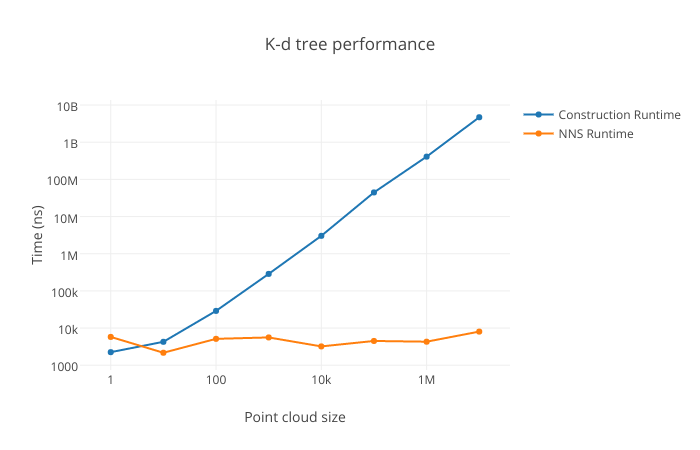
\includegraphics[width=10cm]{results.png}

\section{Analysis}
Our tests revealed that our NNS algorithm is very fast on an already created k-d tree, but
the k-d tree construction is rather inefficient.
This is due to the $O(n \log^2 n)$ behavior of the tree constructor.
The NNS search is not deterministic in its running time as the point cloud and the search
point are random, making it hard to measure well.
However, the running time of the NNS algorithm is so small that there are also other factors
at play, such as clock precision and other programs running on the system.
When many NNS searches are required, using a k-d tree is a good way to cut down on runtime.
Additionally, our NNS search is safe to run in parallel, meaning that a series of worker
threads can be used to speed up large batches of searches on a multiprocessor system.

\section{Code}
The code provided is written in C++14, which requires a compiler with support for it.


\end{document}
